\documentclass[conference]{IEEEtran}

\usepackage{cite}
\usepackage{amsmath,amssymb,amsfonts}
\usepackage{algorithmic}
\usepackage{graphicx}
\usepackage{textcomp}
\usepackage[dvipsnames]{xcolor}
\usepackage{hyperref}
\usepackage{fp}
\usepackage{arydshln}
\usepackage{array}
\usepackage{booktabs}

\newcolumntype{N}{>{\centering\arraybackslash}m{1.31cm}}
\newcommand{\splitcell}[1]{%
	\begin{tabular}{@{}c@{}}\strut#1\strut\end{tabular}%
}
% compare two values to color text
\newcommand{\tabcolor}[2]{{}\FPifgt{#1}{#2}{\textcolor{BrickRed}{#2}}\else{\textcolor{ForestGreen}{#2}}\fi}
% method name in table
\newcommand{\tabn}[1]{  
	\multicolumn{1}{l}{#1}
}
% base, val1, val2, val3 in table
\newcommand{\tabv}[4]{  
	&\tabcolor{#1}{#2}&\tabcolor{#1}{#3}&\tabcolor{#1}{#4}
}

\title{Automatic Skin Labeling of Egocentric Images \\ for Virtual Reality Applications}

\author{\IEEEauthorblockN{1\textsuperscript{st} Heiko Raible}
	\IEEEauthorblockA{\textit{Natural Science and Mathematics} \\
		\textit{h\_da Hochschule Darmstadt}\\
		Darmstadt, Germany \\
		heiko.raible@stud.h-da.de}
}

\begin{document}
\maketitle

\begin{abstract}
Virtual Reality (VR) applications require believable experiences to avoid disorienting users. To achieve this, displaying the user's real body in the virtual environment is a big step forward. However, this can be less believable if the user's clothing does not match the VR environment. To solve this problem, an additional skin class is required in the segmentation step. This paper explores color-based skin segmentation techniques and a deep learning approach to automatically add skin labels to a dataset of egocentric images with body labels. The union of Otsu's method and a histogram-based approach on the HCrCb color space are shown to be effective in a proposed end-to-end system that shows promise as a solution to this problem. A deep learning approach also achieves exceptional performance, although the credibility of it's results is questioned due to a high similarity of the images in the dataset. Future work can improve the robustness and generalizability of the proposed system, and perform a more rigorous evaluation of deep learning approaches.
\end{abstract}

\begin{IEEEkeywords}
virtual reality, egocentric, skin segmentation, mediapipe hands, otsu's method, grabcut, mask r-cnn
\end{IEEEkeywords}

\section{Introduction}

In order for Virtual Reality (VR) applications not to disorient users or make them feel uncomfortable, it is important to make the experience as believable as possible, avoiding anything that might seem out of place. A big step in this direction could be to show them their real body. To achieve this, \cite{b1} has explored placing stereo cameras in front of the Head Mounted Display worn by the user, to segment bodies from egocentric captured videos in real time using deep learning, and then superimpose the body over the image displayed in VR.

This makes the experience more believable in the sense that the user is seeing their own body, but at the same time it can make it less believable by showing their everyday clothes if they don't fit the VR environment. For example, in the case of a medieval VR simulation, it could be very jarring to see the hoodie the user is wearing. To solve this problem, it is necessary to add an additional skin class to the existing body class in the segmentation step. This way, the application can replace the clothing worn, but leave the skin, the actual body of the user, intact.

To train a model for this task, a dataset of egocentric images with both body and skin labels is required, which is highly specific and does not exist in sufficient quality and quantity. Given an existing dataset of egocentric images with body labels, the goal of this work is to create a process to automatically add additional skin labels, which can then be manually improved if necessary.

\section{Research}

\begin{figure*}[h]
	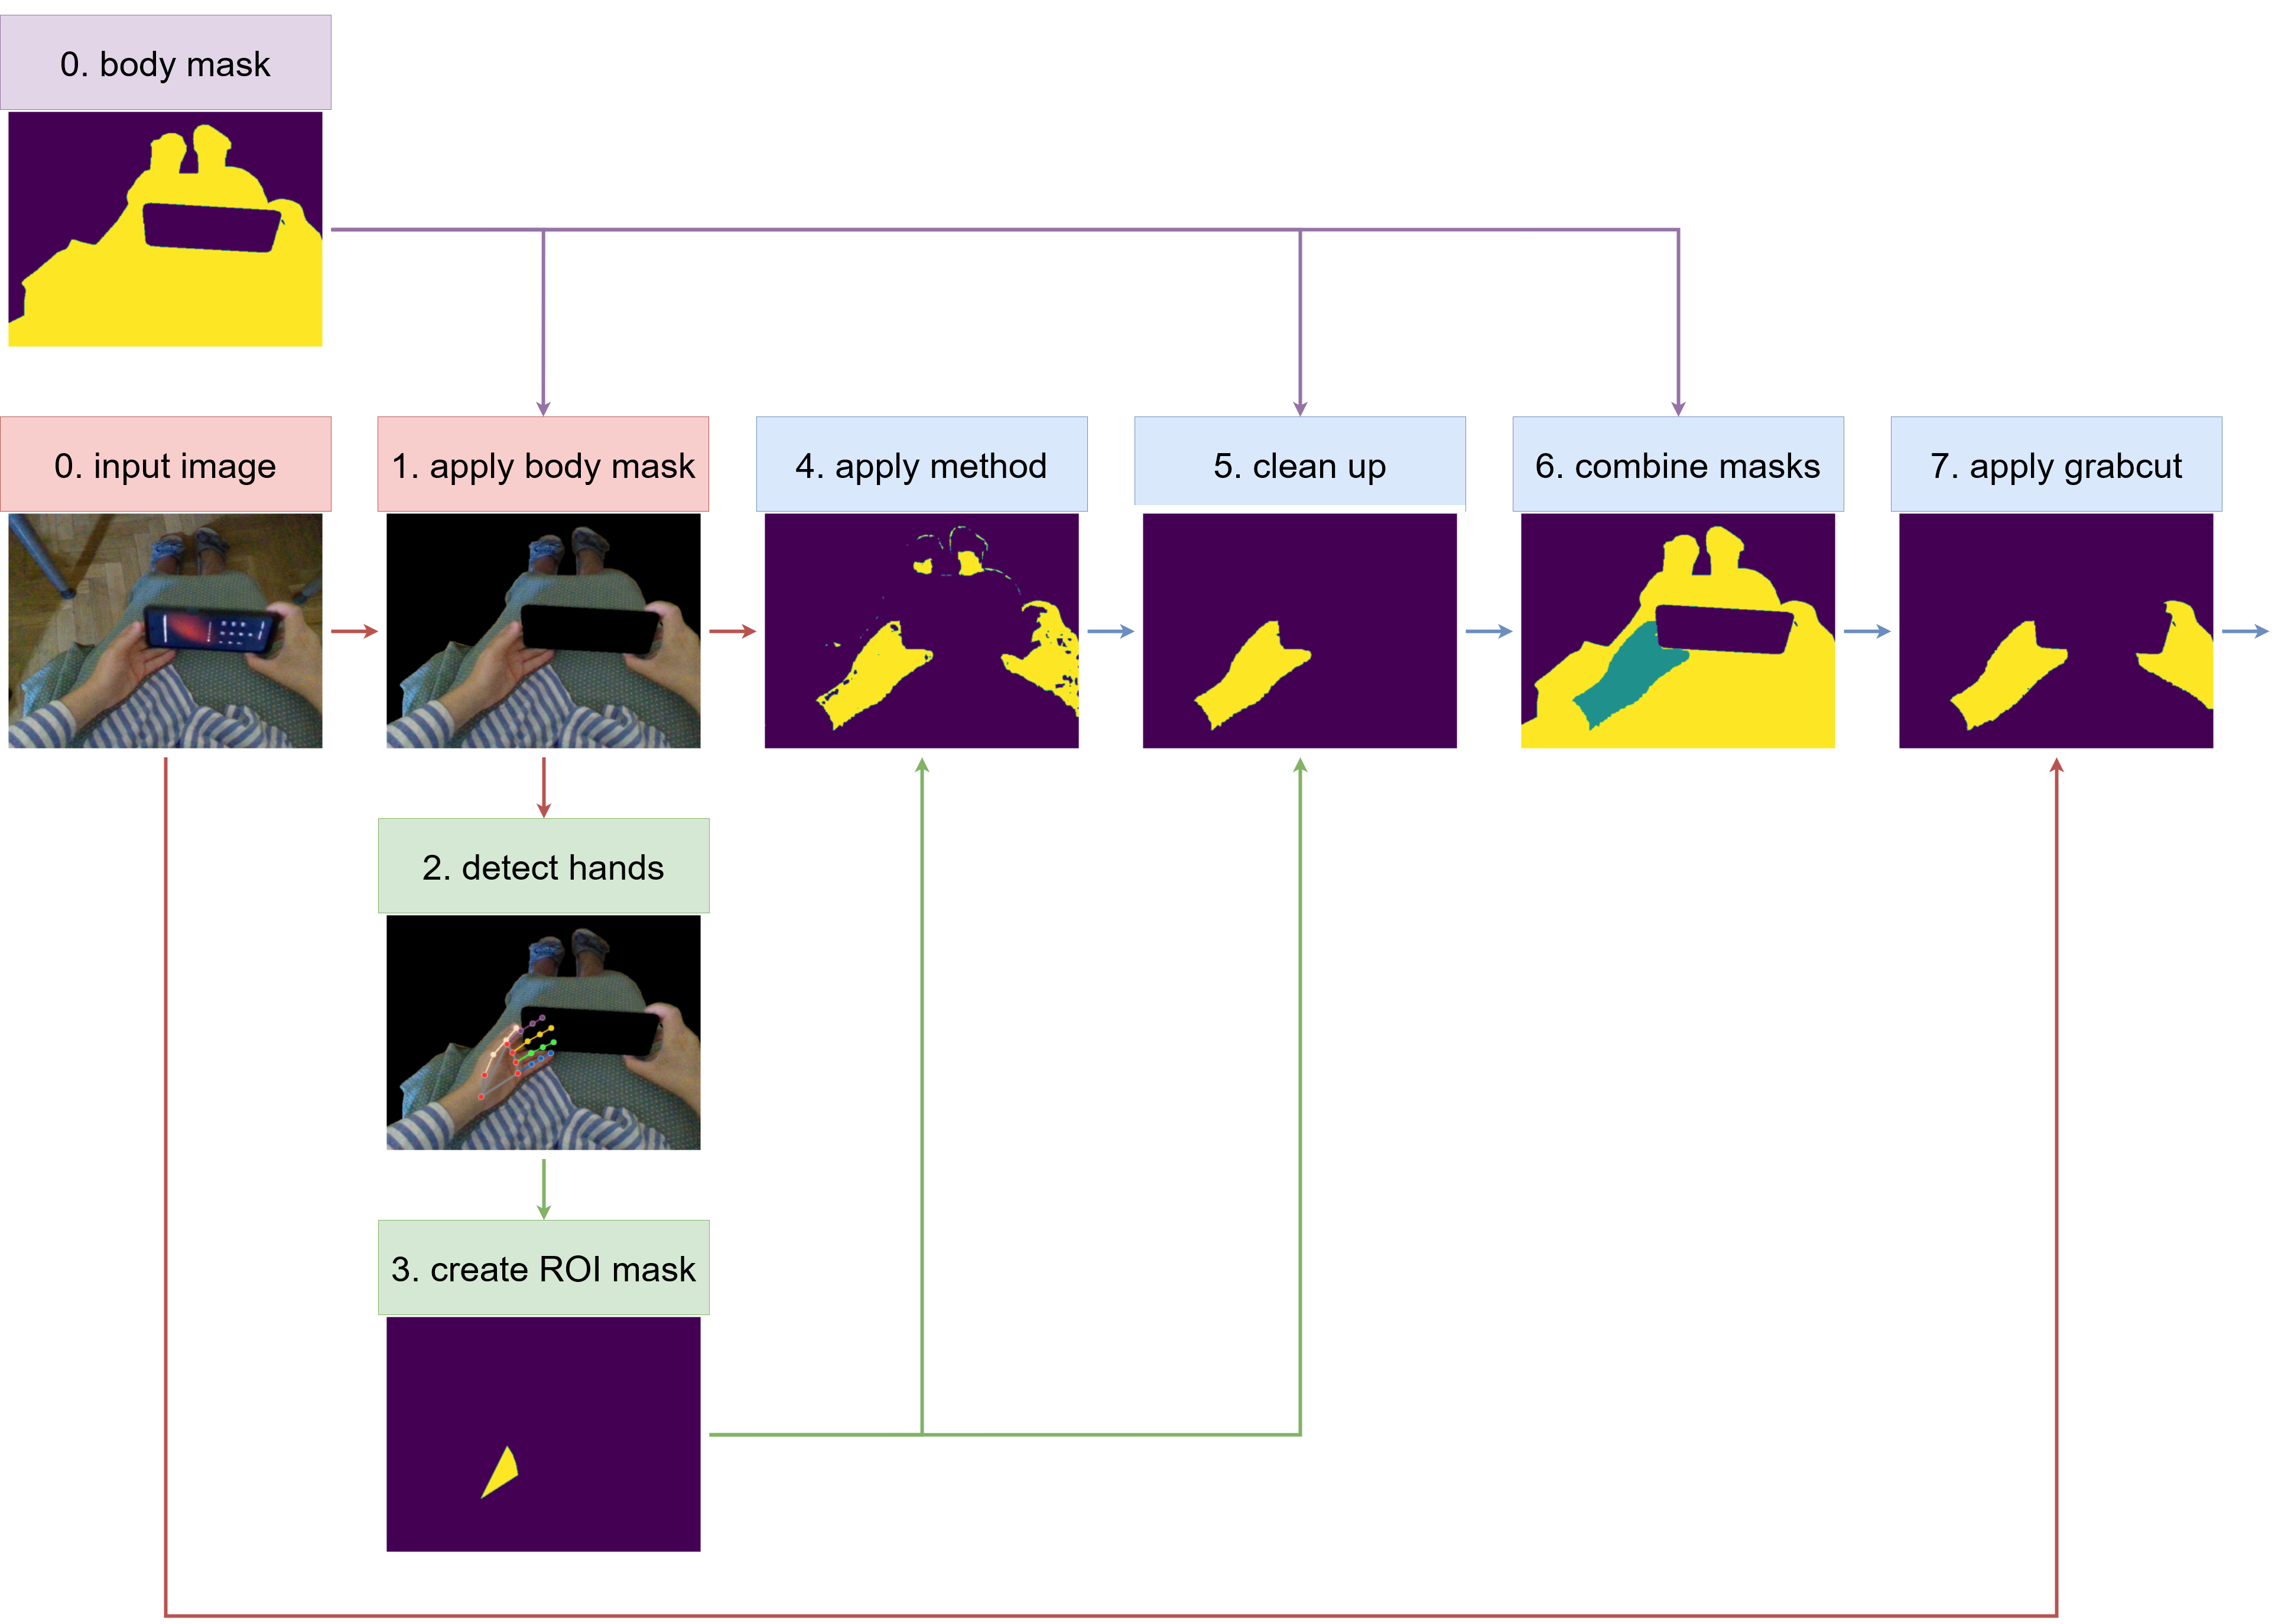
\includegraphics[width=\textwidth]{images/pipeline.png}
	\caption{Graphical representation of the end-to-end system with numbered steps as referenced in section \ref{sec:implementation}.}
	\label{fig:end-to-end system}
\end{figure*}

According to \cite{b2}, the state of the art for color-based skin segmentation is the \textbf{GrabCut} algorithm, introduced in \cite{b3}, which separates a foreground from the background in an image. It is based on graph cuts \cite{b4}, which is an optimization method for finding the minimum cut in a graph. GrabCut requires a rough estimate of the foreground and background regions in the image, and then iteratively refines the segmentation by adjusting the boundary between the foreground and background regions. To do this, it uses two Gaussian Mixture Models to model pixel intensities and also incorporates spatial information to improve segmentation accuracy. The output of the GrabCut algorithm is a binary mask indicating the foreground and background regions in the image. \\

Thresholding can be used in different color spaces to obtain an initial foreground mask to pass to GrabCut. Different color spaces represent colors in different ways, and choosing the appropriate color space can help improve segmentation accuracy \cite{b5}.

The \textbf{RGB} (red, green, blue) color space may not be ideal for segmentation because the color information is tightly coupled with the brightness information, making it difficult to distinguish between objects with similar colors but different brightness levels.

The \textbf{HSV} (hue, saturation, value) color space separates the color information from the brightness information, making it easier to distinguish between objects based on their colors.

The \textbf{YCrCb} (luma, red-difference chroma and blue-difference chroma) color space also separates the color information from the luminance information, again making it more suitable for use in segmentation.

The \textbf{LAB} (lightness, greed-red, blue-yellow) color space again separates color information from lightness. It is designed to be perceptually uniform, meaning that the same distance between two colors in the space is perceived as the same difference in color by the human eye. \\

\textbf{Otsu's method} \cite{b6} is a thresholding technique that aims to find an optimal threshold that separates an image into foreground and background regions based on the intensity (gray scale) values of the pixels. It calculates the variance of the intensity values of the pixels for all possible threshold values between the minimum and maximum intensity values. The threshold that maximizes the between-class variance is selected as the optimal threshold. \\

A novel contribution of this work is the use of \textbf{MediaPipe Hands} \cite{b7}, a lightweight Convolutional Neural Network (CNN) for hand detection based on the MediaPipe framework \cite{b8}, to reliably locate skin patches. Using these skin patches as a region of interest (ROI), it is possible to dynamically determine thresholds in the aforementioned color spaces, in order to effectively segment the image regardless of lighting conditions and skin color. \\

To compare Otsu's method and the MediaPipe Hands-based approach with a deep learning approach, \textbf{Mask R-CNN} \cite{b9} was chosen as a model. Mask R-CNN is a deep learning architecture that extends the Faster R-CNN \cite{b10} object detection model by adding a segmentation task. It can detect and segment objects in an image and generate a binary mask that indicates which pixels belong to each object. The architecture consists of a ResNet \cite{b11} backbone network, a region proposal network for object detection, a region of interest pooling layer for feature extraction, and a mask prediction branch that generates a segmentation mask for each detected object.

\section{Implementation}
\label{sec:implementation}

\begin{table*}[h]
	\begin{center}
		\begin{tabular}{NNNNNNNNNN}\toprule
			\multicolumn{1}{c}{\textbf{}} & \multicolumn{3}{c}{\textbf{THU\_READ\_RGBD} (158 images)} & \multicolumn{3}{c}{\textbf{THU\_READ\_RGBD\_BODIES} (35 images)} & \multicolumn{3}{c}{\textbf{joint-ep-thu-ego} (103 images)} \\
			
			\cmidrule(lr){2-4}
			\cmidrule(lr){5-7}
			\cmidrule(lr){8-10}
			
			\multicolumn{1}{c}{\textbf{thresholding method}} & mIoU (\%) @ method & mIoU (\%) @ clean up & mIoU (\%) @ grabcut & mIoU (\%) @ method & mIoU (\%) @ clean up & mIoU (\%) @ grabcut & mIoU (\%) @ method & mIoU (\%) @ clean up & mIoU (\%) @ grabcut \\
			
			\cmidrule(lr){1-1}
			\cmidrule(lr){2-4}
			\cmidrule(lr){5-7}
			\cmidrule(lr){8-10}
			
			\multicolumn{1}{l}{baseline} & \multicolumn{3}{c}{\textcolor{Dandelion}{81.7}} & \multicolumn{3}{c}{\hspace{-0.41cm}\textcolor{Dandelion}{49.0}} & \multicolumn{3}{c}{\hspace{-0.01cm}\textcolor{Dandelion}{40.3}} \\ \cdashline{1-10} \\
			
			%\tabn{name}										\tabv{base}{val1}{val2}{val3}\tabv{base}{val4}{val5}{val6}\tabv{base}{val7}{val8}{val9}
			\tabn{ROI mask}										\tabv{82.1}{07.4}{07.4}{79.4}	\tabv{49.0}{06.3}{06.3}{77.2}	\tabv{40.3}{09.1}{09.1}{61.4} \\ \cdashline{1-10} \\
			
			\tabn{RGB}											\tabv{82.1}{07.4}{74.5}{75.9}	\tabv{49.0}{08.3}{45.5}{45.8}	\tabv{40.3}{11.0}{31.4}{32.8} \\
			\tabn{HS}											\tabv{82.1}{06.7}{71.0}{76.7}	\tabv{49.0}{07.0}{48.9}{49.7}	\tabv{40.3}{12.7}{48.1}{46.4} \\
			\tabn{CrCb}											\tabv{82.1}{32.1}{74.8}{79.0}	\tabv{49.0}{37.2}{66.9}{65.4}	\tabv{40.3}{29.8}{44.5}{48.1} \\
			\tabn{Otsu's}										\tabv{82.1}{71.8}{67.8}{79.4}	\tabv{49.0}{71.2}{70.3}{77.9}	\tabv{40.3}{47.8}{45.0}{50.5} \\ \cdashline{1-10} \\
			
			\tabn{RGB $\cdot$ HS}								\tabv{82.1}{06.5}{69.7}{76.8}	\tabv{49.0}{06.9}{48.8}{50.1}	\tabv{40.3}{11.8}{44.6}{46.5} \\
			\tabn{RGB $\cdot$ CrCb}								\tabv{82.1}{31.2}{73.6}{79.4}	\tabv{49.0}{36.8}{66.4}{65.5}	\tabv{40.3}{28.0}{42.0}{48.2} \\
			\tabn{HS $\cdot$ CrCb}								\tabv{82.1}{28.7}{68.8}{80.0}	\tabv{49.0}{32.7}{60.1}{69.0}	\tabv{40.3}{28.6}{44.3}{51.6} \\
			\tabn{RGB $\cdot$ Otsu's}							\tabv{82.1}{69.8}{66.5}{79.7}	\tabv{49.0}{70.6}{70.3}{79.0}	\tabv{40.3}{47.9}{44.6}{53.2} \\
			\tabn{HS $\cdot$ Otsu's}							\tabv{82.1}{66.7}{63.1}{79.0}	\tabv{49.0}{63.9}{64.4}{77.3}	\tabv{40.3}{54.5}{48.1}{60.0} \\
			\tabn{CrCb $\cdot$ Otsu's}							\tabv{82.1}{67.6}{65.4}{79.1}	\tabv{49.0}{67.7}{68.3}{77.3}	\tabv{40.3}{53.6}{48.5}{59.4} \\ \cdashline{1-10} \\
			
			\tabn{RGB $\cdot$ HS $\cdot$ CrCb}					\tabv{82.1}{27.8}{67.5}{80.0}	\tabv{49.0}{32.3}{59.5}{69.0}	\tabv{40.3}{26.7}{41.4}{51.8} \\
			\tabn{RGB $\cdot$ HS $\cdot$ CrCb $\cdot$ Otsu's}	\tabv{82.1}{61.9}{60.0}{78.7}	\tabv{49.0}{61.3}{61.9}{77.5}	\tabv{40.3}{49.1}{44.5}{61.9} \\ \cdashline{1-10} \\
			
			\tabn{hist HSV}										\tabv{82.1}{12.9}{11.6}{69.4}	\tabv{49.0}{11.6}{08.6}{73.4}	\tabv{40.3}{23.7}{20.2}{61.0} \\
			\tabn{hist LAB}										\tabv{82.1}{43.1}{43.7}{71.1}	\tabv{49.0}{38.3}{37.5}{71.3}	\tabv{40.3}{47.0}{43.3}{58.8} \\
			\tabn{hist YCrCb}									\tabv{82.1}{41.6}{41.7}{68.3}	\tabv{49.0}{33.1}{32.0}{63.2}	\tabv{40.3}{46.5}{42.9}{59.7} \\
			\tabn{hist HCrCb}									\tabv{82.1}{59.6}{72.1}{80.4}	\tabv{49.0}{60.7}{67.9}{73.2}	\tabv{40.3}{42.5}{49.3}{53.1} \\ \cdashline{1-10} \\
			
			\tabn{hist HCrCb $\cdot$ RGB}						\tabv{82.1}{58.0}{70.7}{80.4}	\tabv{49.0}{59.8}{67.3}{73.2}	\tabv{40.3}{39.6}{46.7}{53.7} \\
			\tabn{hist HCrCb $\cdot$ HS}						\tabv{82.1}{54.6}{65.9}{80.0}	\tabv{49.0}{53.5}{59.9}{73.2}	\tabv{40.3}{39.7}{46.8}{55.7} \\
			\tabn{hist HCrCb $\cdot$ CrCb}						\tabv{82.1}{57.4}{69.6}{79.7}	\tabv{49.0}{58.9}{66.3}{73.7}	\tabv{40.3}{40.7}{47.2}{55.1} \\
			\tabn{hist HCrCb $\cdot$ Otsu's}					\tabv{82.1}{65.9}{63.1}{78.7}	\tabv{49.0}{65.1}{66.1}{77.5}	\tabv{40.3}{58.7}{52.1}{63.4} \\
			\bottomrule
		\end{tabular}
	\end{center}
	\caption{Evaluation of end-to-end system at various stages, per dataset and thresholding method. Red if worse than baseline, green if better.}
	\label{tab:table}
\end{table*}

The full end-to-end system (shown in figure \ref{fig:end-to-end system}) starts with an image and a corresponding body mask as input. In step 1, the body mask is applied to the image, removing all unnecessary information outside the body to simplify the problem. Then, in step 2, MediaPipe Hands is used to detect hands and provide landmark coordinates for `wrist', `index finger', `middle finger', `ring finger', and `pinky', which are then used in step 3 to create a ROI mask for the area between the landmarks. This ROI mask is used in step 4 to determine thresholds in the selected color spaces in different ways: \\

For RGB, HS, and CrCb, the minimum and maximum color values in the ROI were used as thresholds for the entire image. The hue channel in HSV and the luminance channel in YCrCb were ignored. In the case of Otsu's method, the algorithm was applied to the grayscale of the image without using the ROI. Another approach was to look at the histogram of values in the ROI and determine thresholds according to density peaks, which was done in the HSV, LAB, YCrCb, and HCrCb color spaces, the latter consisting of the hue channel of HSV and the red-difference chroma and blue-difference chroma channels of YCrCb. \\

Once the thresholds are determined, they are applied to the masked image to create an initial foreground mask. The union of foreground masks from multiple thresholding methods has also been considered, but only an educated selection of them are evaluated in this paper. In step 4, this foreground mask is then cleaned up by discarding all patches not connected to the ROI mask and and all pixels in the background of the body mask, as well as filling any holes in the remaining mask. The purpose of this foreground mask is to best represent the skin area, and only correct pixels being part of the mask (precision) should take precedence over more of the correct pixels being part of the mask (recall), as it will later be grown using GrabCut. 

In step 6, the cleaned foreground mask is then combined with the body mask by giving the background the value 0 for 'background', the skin the value 1 for 'foreground', and the body the value 2 for 'to be determined'. For the final step 7, the image and this combined mask are given as input to the GrabCut algorithm, which optimizes the 'to be determined' area of the combined mask over several iterations. The resulting mask is the output of the end-to-end system. \\

To compare this end-to-end system with a deep learning approach, a Mask R-CNN was implemented completely separately from this end-to-end system, except that the input images were also masked with the body masks to simplify the problem. The model was pre-trained on the COCO dataset and fine-tuned for 20 consecutive epochs on the dataset described in section \ref{sec:datasets}. The chosen optimization algorithm was Stochastic Gradient Descend with a momentum of 0.9, a weight decay of 5e-4, and a learning rate of 5e-3.

\section{Datasets}
\label{sec:datasets}

\begin{figure}[h]
	\begin{center}
		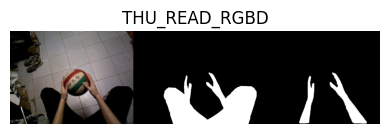
\includegraphics[width=0.5\textwidth]{images/THU_READ_RGBD_example.png} \\
		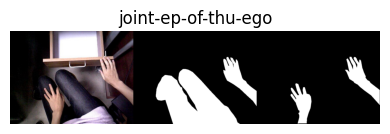
\includegraphics[width=0.5\textwidth]{images/joint-ep-of-thu-ego_example.png}
	\end{center}
	\caption{Example images, body masks and skin masks for datasets.}
	\label{fig:datasets}
\end{figure}

The datasets used were of egocentric scenes showing at least the subject's arms, and contained 158 images for \textbf{THU\_READ\_RGBD} (subset of THU-READ \cite{b12}) and 103 images for \textbf{joint-ep-of-thu-ego} (subset of Egocentric Bodies \cite{b13}), both of which originally had only body labels, but had skin labels commissioned through Amazon Mechanical Turk for evaluation. Example images and masks can be seen in figure \ref{fig:datasets}.

THU\_READ\_RGBD has only 35 images where the body mask contains more than skin, which gives a huge bias towards selecting everything inside the body mask. As a reality check for this dataset, the images containing more than skin were also evaluated separately. THU\_READ\_RGBD also has the disadvantage of having a lot of very similar images because it consists of 5-6 frames from a selection of 32 videos.

Data augmentation would have had no effect on the color-based approach because it treats images separately without any learning process, but it will be applied for Mask R-CNN. \\

The data used for Mask R-CNN is the combination of the two datasets mentioned in the previous paragraph, for a total of 259 images. To augment the dataset, horizontal mirroring was applied, resulting in a dataset of 519 images. To have images that weren't seen in the training process available for evaluation, 200 images were randomly selected for the test dataset, and the remaining 319 images were used for training. It should be noted that most of the images in the dataset have very similar images with slightly different angles or actions, which has not been accounted for in the training of the model.

\section{Evaluation}

The chosen evaluation metric is the Intersection over Union (IoU), which consists of the overlap of the predicted and labeled skin masks, normalized by dividing by the union of the two, displayed in formula \ref{IoU}. To get a comparable value between different thresholding methods for the same dataset, the mean of IoUs (mIoU) is used.

\begin{align}
IOU &= \frac{prediction \cap label}{prediction \cup label}
\label{IoU}
\end{align}

To have a baseline for comparison, the labeled body masks were also directly used as predictions and compared to the labeled skin masks. Because GrabCut is so effective at growing masks against a given background, direct use of the ROI masks was also explored.

To properly evaluate the end-to-end system, the mIoU per dataset was calculated at different points in the pipeline: after the thresholding method, after the clean up, and after GrabCut. The results of this evaluation can be seen in table \ref{tab:table}.

Most thresholding methods improve their mIoU values on each of the steps in the end-to-end system. Throughout the steps you can see that there are a few thresholding methods that stand out: `Otsu's method', `Hist HCrCb', and the unions involving them. The ROI mask and unions of multiple masks generally perform well as foreground masks for GrabCut, showing that precision is prioritized over recall at this stage, which was to be expected. The effect of THU\_READ\_RGBD's bias towards predicting the full body mask is also clearly seen, with the baseline outperforming all other approaches.

The clean up phase increases the mIoU of the previously poorly performing methods, indicating that the thresholds were set too high. It also decreases the mIoU of the previously well-performing methods, which is due to the cases where only one hand is detected even though both are visible, resulting in the discarding of valid skin areas. This is not an issue due to the aforementioned priority of precision and can be remedied in the GrabCut stage. In cases where no hand is detected at all, Otsu's method has an advantage over the others because it doesn't rely on the ROI mask. The evaluation of using the ROI mask directly, which makes huge gains in the GrabCut stage, clearly shows the power of GrabCut. With such a small and simple mask, the results are not far from the best performing approaches, which can be interpreted as the choice of thresholding method not being particularly important. 

\begin{figure}[h]  % maybe 0.5\textwidth
	\begin{center}
		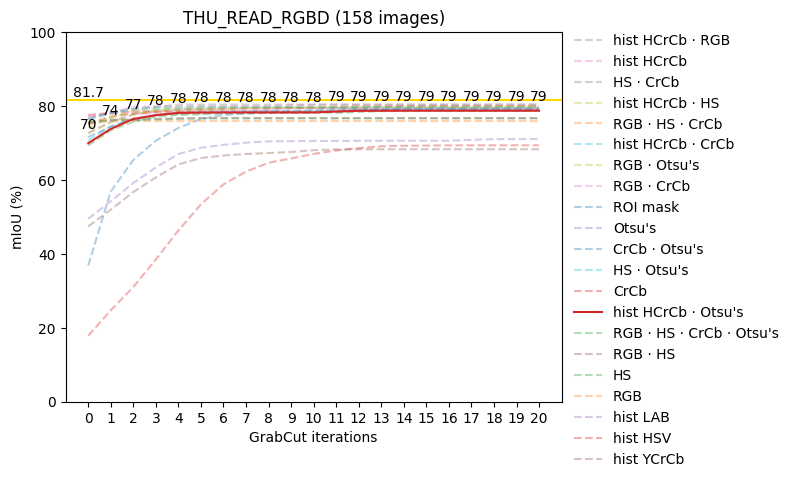
\includegraphics[width=0.45\textwidth]{images/THU_READ_RGBD_grabcut.png}
		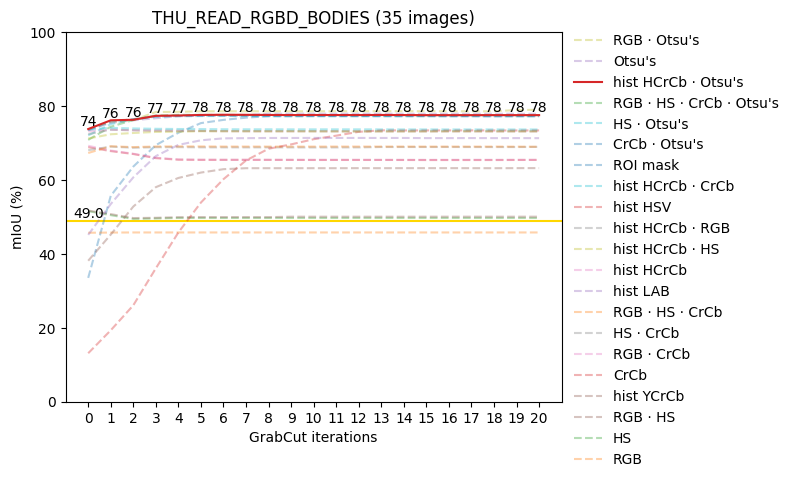
\includegraphics[width=0.45\textwidth]{images/THU_READ_RGBD_BODIES_grabcut.png}
		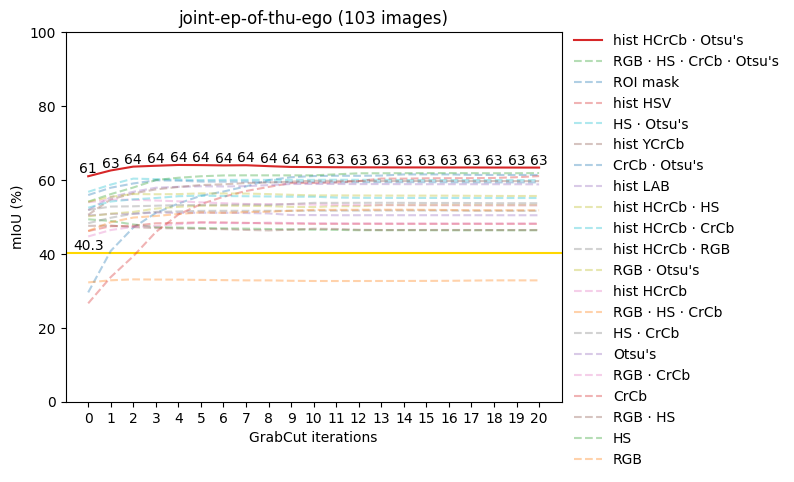
\includegraphics[width=0.45\textwidth]{images/joint-ep-of-thu-ego_grabcut.png}
	\end{center}
	\caption{Evaluation of GrabCut with the most consistent method highlighted in red and the baseline highlighted in yellow.}
	\label{fig:grabcut}
\end{figure}

Since GrabCut is an iterative approach, a range of 20 steps was evaluated. As can be seen in figure \ref{fig:grabcut}, most methods converge around the 5-10th iteration and all are monotonically increasing. Since time is not a constraint for this task, a higher number of iterations is always preferable. The most promising thresholding methods again seem to be the unions containing `Otsu's method` and `hist HCrCb`, with the union of both of them seeming to be the best performing across datasets. \\

\begin{figure}[h]
	\begin{center}
		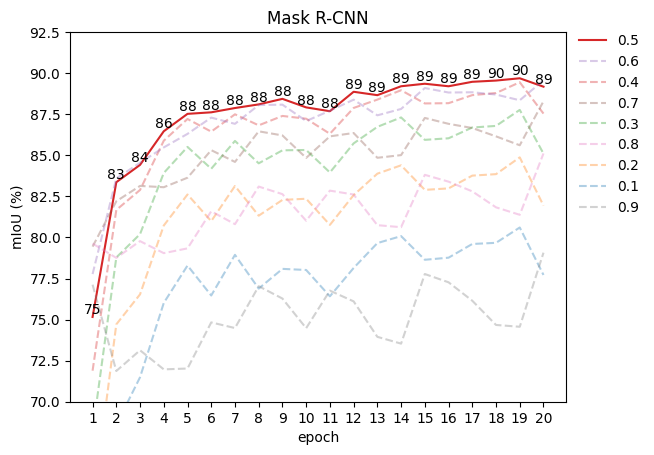
\includegraphics[width=0.45\textwidth]{images/mask_r-cnn.png}
	\end{center}
	\caption{Evaluation of Mask R-CNN epochs and thresholds.}
	\label{fig:MASK R-CNN}
\end{figure}

The evaluation of Mask R-CNN on the 200 separate test images can be seen in figure \ref{fig:MASK R-CNN}. The mIoU increase stagnates around epoch 5 at 88\%, but continues to grow slowly until epoch 19 at 90\%, both with a decision boundary of 0.5. The mIoU of this model is better than the best methods of the end-to-end system, but a comparison is hard to make when taking into account that both datasets were combined and evaluation can only meaningfully take place on a subset of the shuffled data. Most confidence should be given to the 88\% value at epoch 5, where the mIoU increase stagnates, as there is a risk of overfitting due to the high similarity of the images in the dataset. The relative closeness of this mIoU to the best of the end-to-end system could indicate that better results may require better training data. \\

A comparison between hist HCrCb $\cdot$ Otsu's and Mask R-CNN can be seen in figure \ref{fig:results}. They appear to perform similarly, but have their unique failure points. In the first image, the performance is identical. The second image shows the problems that arise when the ROI has very different colors from the rest of the skin due to strong shadows. The third image is an example of what an imperfect dataset can do to a deep learning approach. The collar is mislabeled in the labeling process and learned by the model. This also calls into question the validity of the mIoU values for Mask R-CNN, as there is clearly an overfit on images in the training dataset that are from the same scene as images in the test dataset. The last image might also show an overfit to an image of the same scene in the training dataset with a slightly different angle.

Overall, the best option would most likely be to go with the HCrCb $\cdot$ Otsu's approach when MediaPipe Hands finds a hand, and use Mask R-CNN on the remaining images.

\section{Limitations}

\begin{figure*}[h]
	\begin{center}
		\includegraphics[width=\textwidth]{images/results.png}
	\end{center}
	\caption{Comparison between hist HCrCb $\cdot$ Otsu's and Mask R-CNN.}
	\label{fig:results}
\end{figure*}

The biggest limitation is the aforementioned fact that THU\_READ\_RGBD contains nearly 80\% images where the full body mask is the desired prediction, which is about half of the total data and doesn't represent the use case very well. The data sets aren't perfect either, as many skin masks contain some clothing, among other labeling errors. The aforementioned fact that many images of THU\_READ\_RGBD are very similar also reduces the credibility of it's evaluation, as it effectively reduces the sample size.

Creating a ROI mask with MediaPipe Hands isn't without it's flaws either. If the subject is holding an object, the hand will either not be detected or have non-skin pixels inside the ROI, which can throw off the dynamic thresholding. If only one hand is detected, there may be a loss of correct mask pixels during the clean up stage, which GrabCut will most likely remedy, as seen in the graphical representation of the end-to-end system in figure \ref{fig:end-to-end system}. There are a few images where no hands are detected at all, making it impossible to use all but one of the thresholding methods. This would argue for using Otsu's method or the deep learning approach, which don't require MediaPipe Hands at all, or go with a complimentary approach of using hist HCrCb $\cdot$ Otsu's on the images where MediaPipe Hands can detect hands and Mask R-CNN on the remaining images.

Lastly the dataset used to train the Mask R-CNN is too similar to the images the performance is evaluated on. Performance on a different dataset should be investigated.

\section{Conclusion}

In conclusion, color-based skin segmentation techniques as well as a deep learning approach were explored for the task of automatically adding additional skin labels to a dataset of egocentric images with body labels for virtual reality applications.

Thresholding methods in various color spaces using MediaPipe Hands to determine a ROI as well as Otsu's method were shown to work well for dynamically generating an initial foreground mask for GrabCut. Experiments have shown that using Otsu's method in the proposed end-to-end system or a deep learning approach is more robust in cases where hand detection fails. This work highlights the power of GrabCut for skin segmentation given a body mask, and the proposed end-to-end system shows promise as a solution to this problem, in particular when using hist HCrCb $\cdot$ Otsu's as the thresholding method.

The deep learning approach outperformed the proposed end-to-end system, but the credibility of the results was called into question. Both approaches are complimentary, so the best choice might be to use the end-to-end system with hist HCrCb $\cdot$ Otsu's on the images where MediaPipe Hands can detect hands and Mask R-CNN on the remaining images.

Future work can explore the use of additional datasets and further improvements to the proposed end-to-end system to increase its robustness and generalizability, as well as perform a more rigorous evaluation of deep learning approaches.

\section{Future Work}

Possible iterations upon this work are:

\begin{itemize}
	\item considering the hand detection and/or segmentation of the frame before in video data
	\item being less restrictive between mask and border pixels, since hands always enter an image from the outside
	\item determining if the skin touches the border and apply k-means if it doesn't, with centroids at the hand and border
	\item possibly an additional, different clean up stage after GrabCut
	\item evaluating state-of-the-art semantic segmentation models
	\item using more and/or higher quality datasets
	\item evaluating without GrabCut on datasets without body masks for skin-only dataset creation
	\item evaluating with a generated initial background mask for completely unlabeled skin-only dataset creation, possibly even for lightweight real-time mobile virtual reality applications using only a few GrabCut iterations.
\end{itemize}

\begin{thebibliography}{00}
\bibitem{b1} Gonzalez-Sosa, E., Perez, P., Tolosana, R., Kachach, R., Villegas, A. (2020). Enhanced self-perception in mixed reality: Egocentric arm segmentation and database with automatic labeling. IEEE Access, 8, 146887-146900.

\bibitem{b2} Saxen, F., Al-Hamadi, A. (2014, October). Color-based skin segmentation: An evaluation of the state of the art. In 2014 IEEE International Conference on Image Processing (ICIP) (pp. 4467-4471). IEEE.

\bibitem{b3} Rother, C., Kolmogorov, V., Blake, A. (2004). "GrabCut" interactive foreground extraction using iterated graph cuts. ACM transactions on graphics (TOG), 23(3), 309-314.

\bibitem{b4} Boykov, Y. Y., Jolly, M. P. (2001, July). Interactive graph cuts for optimal boundary \& region segmentation of objects in ND images. In Proceedings eighth IEEE international conference on computer vision. ICCV 2001 (Vol. 1, pp. 105-112). IEEE.

\bibitem{b5} Leite, M., Parreira, W. D., Fernandes, A. M. D. R., Leithardt, V. R. Q. (2022). Image Segmentation for Human Skin Detection. Applied Sciences, 12(23), 12140.

\bibitem{b6} Otsu, N. (1979). A threshold selection method from gray-level histograms. IEEE transactions on systems, man, and cybernetics, 9(1), 62-66.

\bibitem{b7} Zhang, F., Bazarevsky, V., Vakunov, A., Tkachenka, A., Sung, G., Chang, C. L., Grundmann, M. (2020). Mediapipe hands: On-device real-time hand tracking. arXiv preprint arXiv:2006.10214.

\bibitem{b8} Lugaresi, C., Tang, J., Nash, H., McClanahan, C., Uboweja, E., Hays, M., ... Grundmann, M. (2019). Mediapipe: A framework for building perception pipelines. arXiv preprint arXiv:1906.08172.

\bibitem{b9} He, K., Gkioxari, G., Dollár, P., Girshick, R. (2017). Mask r-cnn. In Proceedings of the IEEE international conference on computer vision (pp. 2961-2969).

\bibitem{b10} Ren, S., He, K., Girshick, R., Sun, J. (2015). Faster r-cnn: Towards real-time object detection with region proposal networks. Advances in neural information processing systems, 28.

\bibitem{b11} He, K., Zhang, X., Ren, S., Sun, J. (2016). Deep residual learning for image recognition. In Proceedings of the IEEE conference on computer vision and pattern recognition (pp. 770-778).

\bibitem{b12} Tang, Y., Wang, Z., Lu, J., Feng, J., Zhou, J. (2018). Multi-stream deep neural networks for rgb-d egocentric action recognition. IEEE Transactions on Circuits and Systems for Video Technology, 29(10), 3001-3015.

\bibitem{b13} Gonzalez-Sosa, E., Gajic, A., Gonzalez-Morin, D., Robledo, G., Perez, P., Villegas, A. (2022). Real time egocentric segmentation for video-self avatar in mixed reality. arXiv preprint arXiv:2207.01296.

\end{thebibliography}
\end{document}
